\documentclass{esannV2}
\usepackage[utf8]{inputenc}
\usepackage{natbib}
\usepackage{graphicx}
\usepackage{float}

%***********************************************************************
% !!!! IMPORTANT NOTICE ON TEXT MARGINS !!!!!
%***********************************************************************
%
% Please avoid using DVI2PDF or PS2PDF converters: some undesired
% shifting/scaling may occur when using these programs
% It is strongly recommended to use the DVIPS converters, and to submit
% PS file. You may submit a PDF file if and only if you use ADOBE ACROBAT
% to convert your PS file to PDF.
%
% Check that you have set the paper size to A4 (and NOT to letter) in your
% dvi2ps converter, in Adobe Acrobat if you use it, and in any printer driver
% that you could use.  You also have to disable the 'scale to fit paper' option
% of your printer driver.
%
% In any case, please check carefully that the final size of the top and
% bottom margins is 5.2 cm and of the left and right margins is 4.4 cm.
% It is your responsibility to verify this important requirement.  If these margin requirements and not fulfilled at the end of your file generation process, please use the following commands to correct them.  Otherwise, please do not modify these commands.
%
\voffset 0 cm \hoffset 0 cm \addtolength{\textwidth}{0cm}
\addtolength{\textheight}{0cm}\addtolength{\leftmargin}{0cm}

%***********************************************************************
% !!!! USE OF THE esannV2 LaTeX STYLE FILE !!!!!
%***********************************************************************
%
% Some commands are inserted in the following .tex example file.  Therefore to
% set up your ESANN submission, please use this file and modify it to insert
% your text, rather than staring from a blank .tex file.  In this way, you will
% have the commands inserted in the right place.

\begin{document}
%style file for ESANN manuscripts
\title{Towards metacognitive agents: integrating confidence in sequential decision-making}

%***********************************************************************
% AUTHORS INFORMATION AREA
%***********************************************************************
\author{B. Pesquet$^1$ and F. Alexandre$^1$
%
% Optional short acknowledgment: remove next line if non-needed
% \thanks{This is an optional funding source acknowledgement.}
%
% DO NOT MODIFY THE FOLLOWING '\vspace' ARGUMENT
\vspace{.3cm}\\
%
% Addresses and institutions (remove "1- " in case of a single institution)
1- INRIA, University of Bordeaux, CNRS, Bordeaux INP - France
%
% Remove the next three lines in case of a single institution
% \vspace{.1cm}\\
% 2- School of Second Author...
}
%***********************************************************************
% END OF AUTHORS INFORMATION AREA
%***********************************************************************

\maketitle

\begin{abstract}
In natural cognition, confidence is used to evaluate the quality of decisions and adapt one's behavior to the task at hand. For now, artificial agents lack this kind of metacognitive ability and interact with their environment in a purely reactive way. Inspired by recent findings about the cognitive modeling of confidence, we propose a novel architecture for sequential decision-making. It combines an evidence accumulation model with a metacognitive module that computes and exploits confidence to tune the decision process. The model has been assessed on a perceptual decision-making task, showing promises for more flexible artificial agents and a possible path towards artificial metacognition.

\end{abstract}

\section{Introduction}

Everyday, we make a myriad of choices regarding many topics, big and small. Decision-making, the cognitive process leading to a decision, is one of the key skills to adapt to one's environment and reach one's goals. At the cognitive level, a number of these decisions are taken in a reactive and implicit way, using knowledge and associations learned through previous experiences. For example, when asked if $2+2=5$, chances are you would answer immediately without any explicit reasoning. But some other decisions are tougher to make, either because of the imperfections in the information guiding the choice, or because of the stakes involved \cite{flemingMetacognitionConfidenceReview}. Imagine, for example, that you are preparing yourself for an upcoming test. Before the big day, deciding whether or not you understand the material well enough to stop studying is not an easy choice to make. After taking the test, you might reflect (more or less anxiously) on your answers, trying to assess your performance level. Both cases imply a form of self-evaluation regarding your cognitive processes and an explicit deliberation which might inhibit a too simple reactive decision and promote instead a contextually more adapted decision. The ability to reflect on, evaluate and control one's mental functions is called \textit{metacognition}. This practice of "thinking about thinking" is a key skill to adapt to complex problems and changing environments.

Concerning the first aspect of reactive and implicit decision making, Artificial Intelligence (AI) has proposed several approaches, including reinforcement learning with a slow learning based on reward prediction errors. Similarities at both the behavioral and computational levels have been reported with reactive decision making in animals \cite{suri_neural_1999}. AI has only recently begun to consider explicit and deliberative decision making, mainly by proposing ways to emulate deliberation, like with Chain-of-Thought prompting in Large Language Models \cite{wei_chain--thought_2024}. Yet, this kind of method is still very preliminary, with an unreasonable computational cost and far from some human characteristics (e.g., flexibility, explainability) \cite{lake_building_2017}. In addition, the stage of self-evaluation playing a major role before the explicit control of cognitive processes is largely neglected in modern AI.

Another line of research more associated with experimental psychology has proposed to explicitly model the sequential deliberative process of decision making as accumulation of evidence \cite{ratcliff_diffusion_2016}. Initially designed for binary choices and not considering the learning phase, this model family has been extended to ease the implementation of coupled learning and decision in cognitive agents \cite{van_ravenzwaaij_accumulating_2020} and studies to assess its biological plausibility have been proposed \cite{nallapu2024}. Such models are very interesting because they can provide quantitative explanations of psychometrics and chronometrics of decision making, but under the condition that an accepted error rate can be given a priori to the model.

Artificial agents lack the capacity to reflect upon themselves, to question their choices and behaviors. Augmenting them with metacognitive abilities could be essential to improve their performance, but also their acceptability. In particular, the ability to evaluate one's ability to make a decision, that is also called confidence, is a necessary step. A simple but efficient way of implementing such a mechanism in a sequential decision process is described below and evaluated on a simple perceptual task.

\section{Related work}

\subsection{Sequential decision-making}

A decision is a deliberative process that results in the commitment to a categorical proposition \cite{goldNeuralBasisDecision2007}. Decision making is generally a \textit{sequential} process, either because we need time to collect informative cues, one after the other (like a detective collecting pieces of evidence) or because we need time to process each cue, one after the other (like a chess player). 

A popular class of models assumes that a decision maker accumulates pieces of evidence for each alternative until a threshold is reached for one alternative. Such accumulation-to-threshold models are known as \textit{sequential sampling models} or \textit{evidence accumulation models} (EAM). One of the first and most popular EAMs is the Diffusion Decision Model (DDM), also called Drift-Diffusion Model, originally designed in the 1970's \cite{Ratcliff1978ATO} to study binary choices.

This class of models is used to study the time constraints of decision by accumulation \cite{forstmannSequentialSamplingModels2016}. The intuitively understandable balance between response time and accuracy is called the \textit{speed/accuracy trade-off} (SAT) \cite{heitzSpeedaccuracyTradeoffHistory2014}.

In their simplest form, evidence accumulation models have three parameters: the boundary separation $a$ that implements the SAT, the starting point $z$ that represents the pre-decision bias in favor of one of the responses, and the drift rate $v$ that models the speed of evidence accumulation processing.

\begin{figure}
    \centering
    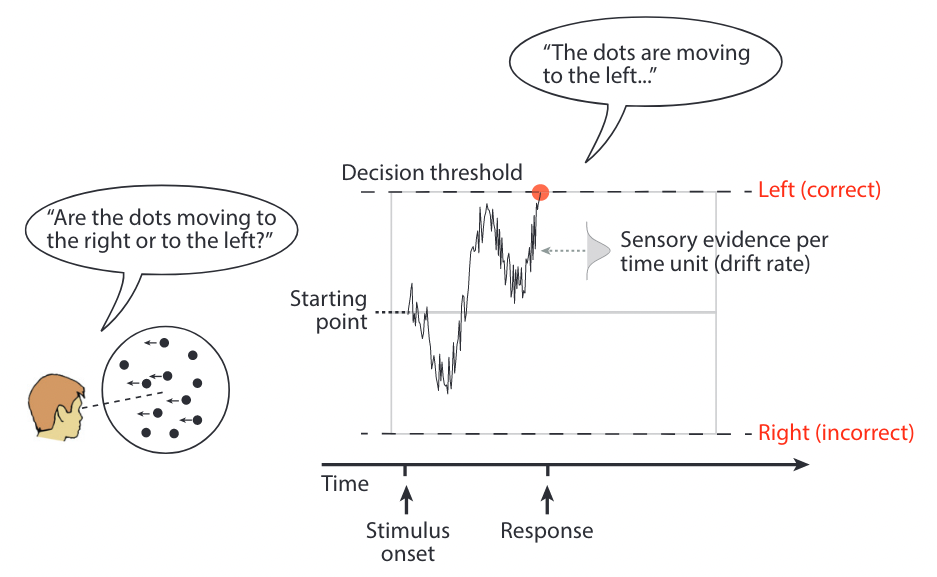
\includegraphics[width=0.7\linewidth]{images/forstmannSequentialSamplingModels2016.png}
    \caption{Illustration of the Diffusion Decision Model \cite{forstmannSequentialSamplingModels2016}}
    \label{fig:ratcliff-ddm}
\end{figure}

Many subsequent works have refined this seminal model to account for multiple choices \cite{vanravenzwaaijAccumulatingAdvantagesNew2020}, change of mind \cite{resulajChangesMindDecisionmaking2009} or impacts of learning on the decision outcome \cite{fontanesiReinforcementLearningDiffusion2019}, \cite{mileticNewModelDecision2021}.

\subsection{Confidence in decision-making}

Everyone knows intuitively what confidence is about, yet it is seldom defined explicitly. In the broadest sense, confidence quantifies a degree of belief in something or someone \cite{meynielConfidenceBayesianProbability2015}, where a belief can be defined as a feeling of certainty about a proposition (i.e. a statement or a decision). It is a subjective, conscious experience. Confidence is fundamentally linked to its object: a thought, a choice, an external actor, etc.

In decision-making, confidence can be seen as the subjective estimate of decision quality \cite{brusSourcesConfidenceValuebased2021}.  More formally, it can be defined as the probability that a choice is correct given the evidence \cite{pougetConfidenceCertaintyDistinct2016}. Confidence is a form of certainty. A key difference is that contrary to confidence, (un)certainties are decision independent \cite{flemingMetacognitionConfidenceReview}. Confidence quantifies the degree of certainty associated with a decision.

When using an evidence accumulation model to study the decision process, a simple and natural way of evaluating confidence is by computing the difference between accumulators for each alternative. The larger the gap, the higher the confidence should be, reflecting a more robust decision. Furthermore, this approach is biologically grounded \cite{kepecsNeuralCorrelatesComputation2008}.

\section{Proposed model}

Taking into account the previous literature on confidence and human decision-making, we designed a model for an artificial agent including two components:
\begin{itemize}
    \item A \textit{decision module} which uses an evidence accumulation model to select the chosen alternative.
    \item A \textit{metacognitive module} which tunes the decision process through adjusting the decision hyperparameters (threshold and rate of evidence integration; the starting point is not considered in the task here).
\end{itemize}

The decision module's evidence accumulation is based on a \textit{race model}. Evidence favoring each alternative is accumulated separately, and the decision is taken once the first accumulator reaches the threshold.

The metacognitive module uses the difference between accumulators to compute the confidence associated with the decision. Confidence is then used to tune the decision process, implementing the metacognitive ability of switching between different strategies. For example, detecting a low confidence value should trigger a more cautious approach and consequently a longer time of evidence accumulation; conversely, being more confident should lead to a quicker decision.

 \begin{figure}[H]
     \centering
     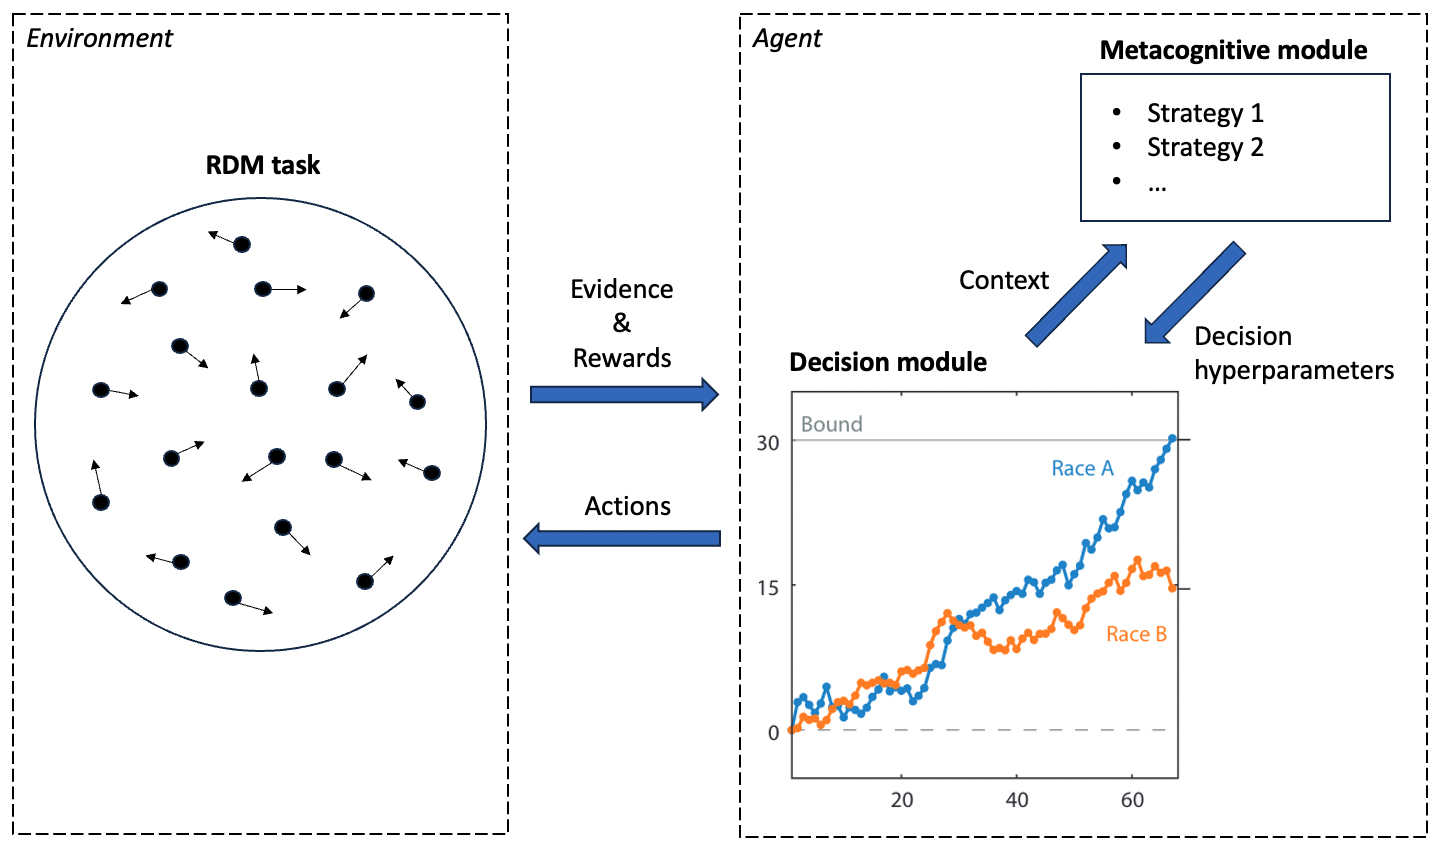
\includegraphics[width=1\linewidth]{images/confident_agent_architecture.png}
     \caption{Task and agent model}
     \label{fig:agent-architecture}
 \end{figure}

The model was trained on an adaptation of the Random Dot Motion (RDM) task. This well-known psychophysical experiment continuously presents a set of moving dots to the subject, who has to make a decision regarding their movement: do the majority of dots move to the left or to the right? The experimenter can modulate the difficulty of the task through several factors, notably the coherence of the dot cloud (percentage of dots moving in the same direction).

\section{Experimental validation}

The model was implemented in Python and trained on a custom Gymnasium environment mimicking the RDM task. Two variations of the task were used: one with a strong coherence between dots and another with more random movements.

At each timestep of a training episode, information about dots is provided to the model as raw pixel values. Integrating this evidence in the corresponding accumulator, the agent can decide to wait for more data or make a decision regarding the dot movement (which ends the episode). After each episode, rewards are considered a posteriori by the model to adjust the metacognitive process.

The first results demonstrate how the metacognitive module alters the decision process. They indicate that the agent model is able to implement a Speed-Accuracy Tradeoff \cite{heitzSpeedaccuracyTradeoffHistory2014}, a hallmark of human cognition.

\begin{figure}[H]
    \centering
    \subfigure(a){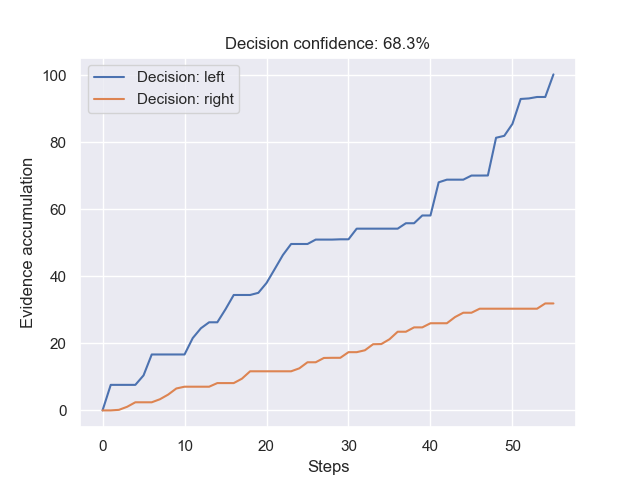
\includegraphics[width=0.45\textwidth]{images/confidence_high.png}}
    \subfigure(b){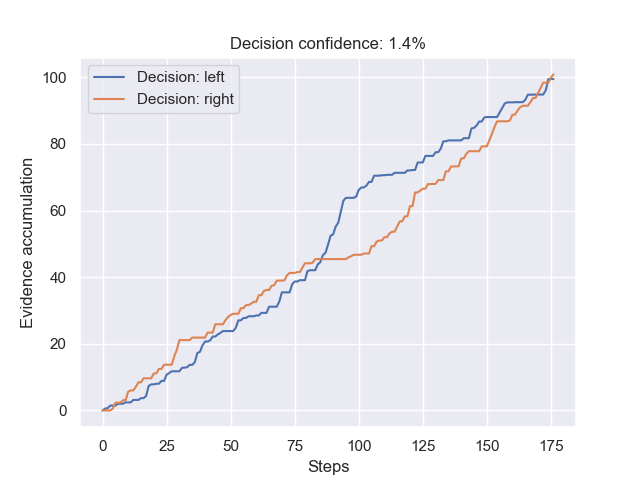
\includegraphics[width=0.45\textwidth]{images/confidence_low.png}}
    \caption{Experimental results. (a) Easy environment: high confidence and short decision process. (b) Harder environment: low confidence and longer process.}
    \label{fig:results}
\end{figure}

\section{Conclusion and perspectives}

Human decision-making is of sequential nature and characterized by our ability to reflect upon ourselves and adapt our behavior accordingly. A growing body of work at the crossroads of psychology and computational neuroscience studies the role of confidence in the decision process, and its formation in the brain.

Drawing from these premises, we defined a model for a metacognitive artificial agent able to evaluate its confidence and use it to adapt its decision process on-the-fly. We tested this model on a classic perceptual decision task. First results show the positive (and expected) impact of metacognition on the agent's behavior.

 Ongoing works are carried out to consolidate the first results regarding confidence evaluation and use in decision making. Further developments will be needed to refine and extend the cognitive architecture to more general aspects of metacognition, towards autonomous and flexible behavior of an artificial agent.

% ****************************************************************************
% BIBLIOGRAPHY AREA
% ****************************************************************************
\begin{footnotesize}

\bibliographystyle{unsrt}
\bibliography{biblio}

\end{footnotesize}

% ****************************************************************************
% END OF BIBLIOGRAPHY AREA
% ****************************************************************************

\end{document}
